\section{A Model of Unrecognized Statehood} 
We model a dispute over a piece of territory that is controlled by a secessionist group and also claimed by a home state. The central issue of contention, independence vs. reunification, is both difficult to divide and highly valued by both sides. The side payments that can be offered in exchange for the opponent's surrender of the independence/reunification issue are sharply limited by the absence of large concessions that can credibly be made (Walter 1997, 2002; Schultz 2010).

Because our model incorporates the incentives and actions of international actors, it is about to both articulate the mechanisms that create these persistent stalemates and to assess the consequences, intended and otherwise, of outside actors' attempts to foster their desired outcome.\footnote{For another example of the strategic manipulation of decision-makers into (and out of) conflict see Baliga and Sjostrom (2012).}

\subsection{The Players}

We construct a model with four players: the secessionist elite ($s$), which seeks recognized independence; the central government of the home state ($g$) from which $s$ is attempting to secede, which seeks reunification; and two outside actors:the patron ($p$) and the international community ($c$).

Player $c$ prefers reunification to recognized independence---a preference that is common to most states, and especially among those that fear the prospect of secessionist movements within their own borders. In practice we often observe groups of states like the OECD or the UN acting in this capacity.

Player $p$ most prefers recognized independence, aligning its interests with the secessionists. We refer to $p$ as the patron because $p$ contributes resources to the unrecognized state in the status quo equilibrium. Patrons choose to contribute resources to secessionists for one or more of several reasons: 1) As an efficient mechanism for imposing costs on the home state (Salehyan et al., 2012), e.g. as Russia does to Georgia via South Ossetia and Abkhazia; 2) ethnic solidarity with the secessionists (e.g. Turkey's support of the Turkish Republic of Northern Cyprus); 3) hope of eventual annexation of the disputed territory (e.g. Armenia's support of Nagorno-Karabakh). Although there may exist patrons whose most-preferred outcome is the status quo, we examine the case where the patron's most preferred outcome is independence because this is the condition under which the status quo is least likely. We will show that even in this circumstance the status quo remains an equilibrium outcome.

\textbf{<<COMP: Place Figure 1 about here>>}

\subsection{Details of the Dynamic Game}
\label{sec:structure}

The game begins at a status quo in which the secessionist elite controls at least some of the disputed territory but cannot gain international recognition unless the central government cedes its claim to the territory. This condition is archetypical of cases in which a militarily successful war of secession ends in a ceasefire.  

There are an infinite number of discrete periods $t=1,2,\ldots$. Play proceeds in each period $t$ as follows (and as shown in Figure 1) until an absorbing state is reached.

\begin{enumerate} 
\item $p$ chooses an investment level to influence the payoffs of $s$ and $g$. 
 
\item $c$ chooses an investment level to influence the payoffs of $s$ and $g$.
 
\item Conflict Stage Game: $s$ and $g$ play a stage game in which each chooses simultaneously from the following actions: Fight, Status Quo, Cede. 
\end{enumerate}

The payoffs at the end of a period are determined by these actions and six state variables. These state variables keep track of the value of the status quo, losing and winning the issue of status for the secessionists and government respectively. 

The game continues into the next period if the `inside players'---the secessionists and government---selected (status quo, status quo) or (cede, cede). Otherwise, the game ends in an absorbing state as described in Section~\ref{sec:stage}.

Future payoffs are discounted with a common parameter $\de \in [0,1]$. Therefore payoffs for the entire game for player $i\in \{s, g, p, c\} $ can be expressed by the discounted stream of payments $\Sigma_{t=1}^{\infty} \de^{t-1} U_i^t $ where $U_i^t$ is player $i$'s payoff in period $t$.

The payoff functions and all parameters, including probabilities in the war lottery, are common knowledge for all players.


\subsubsection{Within-period Payoffs for the Secessionists and Government}
\label{sec:stage}

\noindent Payoffs for players $s$ and $g$ in period $t$, gross of investments by players $p$ and $c$, are:
\vspace{2pt}
\textbf{<<COMP: Place Figure 2 about here>>}
\vspace{2.5pt}

All the state variables except for the secessionists' status quo payoffs remain unchanged from period to period unless players $p$ or $c$ make an investment. To be precise, we have\footnote{Here we anticipate a bit the incentives of the patron and international community to sign the impact of contributions in each case.}
	\begin{equation}
	\begin{aligned}
		L_s^t = L_s^{t-1} - R_p^t + R_c^t \hskip.5in L_g^t = L_g^{t-1} + R_p^t - R_c^t \\
		W_s^t = W_s^{t-1} + R_p^t - R_c^t \hskip.5in W_g^t = W_g^{t-1} - R_p^t + R_c^t \\
		Q_g^t = Q_g^{t-1} - R_p^t + R_c^t \hskip.5in Q_s^t = Q_s^{t-1} - \mu + R_p^t - R_c^t
		\label{eqn:motion}
	\end{aligned}
	\end{equation}
	

The status quo payoffs for the secessionists are special in that the transition of this state variable from one period to the next involves an automatic reduction by $\mu$. The steady reduction by $\mu$ represents the costs of non-recognition discussed in the introduction.

Only two outcomes of the stage game do not lead to absorbing states, and the payoffs for these are bolded. If both $s$ and $g$ play Status Quo, then the status quo persists. Likewise, if both states simultaneously play Cede, we assume that both renege immediately and that the status quo is preserved for that period. In this case neither player has demonstrated a willingness to give up more than the other. Therefore, payoffs for both players ceding simultaneously are identical to the status quo payoffs.%\footnote{This assumption is appropriate as precise simultaneity is an artifact of discrete time modeling: it is not a phenomenon we observe in the real world.} 

If either $s$ or $g$ plays Cede while the other plays Fight or Status Quo, the game enters an absorbing state (i.e. the game ends), with payoffs in every subsequent period given by the corresponding entry in the stage game (Figure 2). We interpret one player ceding as that player ceding the issue of status (independence vs. reunification) in exchange for some set of (relatively small) payments from the opposing player. Therefore, if one player agrees to cede while the other player chooses to remain in the status quo or fight, the result is a negotiated settlement benefiting the player who did not cede. 

There are three ways to end up in war: either of the parties may attack first, or both may attack simultaneously. We denote the payoffs of war as a lottery $\Omega$. This lottery determines whether the secessionists or government wins the war. For simplicity, we assume the outcome of the war is an absorbing state. Outright victory would, among other things, allow an unrecognized state to force recognition by the home state government.

For probabilities $p$ of outright victory and $1-p$ of loss, player $i \in \{s, g\}$ in period $t$ with a fixed cost of war $\zeta_i$ faces war lottery $\omega_i^t \equiv (p (W_i^t-\zeta_i), \left(1-p\right)( L_i^t-\zeta_i))$. $\Omega^t \equiv (\omega_g^t, \omega_s^t).$ Players are assumed to approach war lotteries as expected values.

We do not restrict the preferences and capabilities for players $g$ and $s$, with one exception. We assert that the payoffs for the party that cedes the issue of status (independence vs. reunification) are consistently low. This reflects the fact that the issue of status is indivisible and highly valued by each side and that many of the payments that could be offered are not credible (Licklider, 1995; Walter 1997, 2002; Doyle and Sambanis, 2006; Fearon and Laitin, 2007; Schultz, 2010).



\subsubsection{Within-period Payoffs for the Patron and International Community}
We assume player $c$ prefers peace to war. For simplicity, we limit our modeling of $c$'s preference for peace to the assumption that $c$ will not choose to fund a military buildup that it expects will induce war. This assumption is not necessary for the basic results to hold; however, it justifies our decision not to address military support of armed reconquest by the home state as a deliberate strategy by $c$ to achieve reunification. 

We use two binary variables to express the preferences among the three outcomes (status quo, reunification, recognition by the home state) for both $p$ and $c$. $X$ represents reunification: $X=0$ in the status quo and $X=1$ if the secessionists rejoin the home state. Y represents recognition: $Y=1$ if the home state recognizes the secessionists as independent, $Y=0$ otherwise. 

Player $p$'s payoffs in period $t$ are $U_p^t= -\alpha X+\lambda Y -R_p^t$, while the payoffs for player $c$ are $U_c^t= \beta X-\nu Y -R_c^t$, with both payoffs denoted in currency units. Taking $\alpha, \ \beta, \lambda,$ and $\nu$ to be positive, these payoffs represent the idea that the patron opposes reunification while player $c$ prefers it, and that the patron prefers recognized independence while player $c$ is averse to the creation of new states.



\section{Explaining Outcomes of Secessionist Conflicts} 
\label{sec:main}
%The game has three outcomes that we will consider, each of which can be characterized by a class of equilibria. The outcome of greatest interest is both players choosing the status quo in perpetuity; we will also examine the two absorbing states, reunification and recognition by the home state (i.e. recognized statehood).\footnote{Other classes of equilibria are possible, for example it is theoretically possible for the players to agree to a lottery between the absorbing states which would yield a higher expected payoff than the status quo. However, in practice there is a credibility issue: the losing party does not have an incentive to cede if they lose the lottery. Such strategies are, in any case, not analyzed here.} 

Despite the preferences of the international community for peace, the most common outcome of secessionist conflicts in the post-WWII period has been reunification with the home state via outright military reconquest. By contrast, reunification through negotiated settlement has been very rare. We will explore potential explanations for this seeming inability of the international community to achieve its aims in Section~\ref{sec:alt}. First, we turn to the outcome that we find the most puzzling: perpetual unrecognized statehood.

\subsection{The ``Status Quo'' Equilibrium} 
\label{sec:mainproof}
Unrecognized states are frequently viewed as temporary phenomena or as non-equilibrium outcomes attributable to players' misperceptions of the strategic situation, or their fundamental irrationality. Our central result shows that unrecognized statehood can be an equilibrium outcome capable of being sustained in perpetuity by fully rational, perfectly informed actors. 

We begin by listing and providing intuition for a set of restrictions on the preferences of the actors and their resources for which we can guarantee that unrecognized statehood is an equilibrium outcome. This set of restrictions identifies a class of games, $\mathcal{G}$: 

\begin{definition}
\emph{The class $\mathcal{G}$ includes all those games for which following restrictions are satisfied:}

\begin{enumerate}
\item \textit{For both players $g$ and $s$, remaining in the status quo is better than ceding at the beginning of the game.}\label{res:1}

\item \textit{For both players $g$ and $s$, the expected outcome under war is worse than the status quo at the beginning of the game.}\label{res:2}

\item \textit{Either the secessionists prefer ceding to war or the patron's disutility from war is greater than the per-period cost of offsetting the deterioration in the secessionists' status quo payoffs.}\label{res:new}

\item \textit{Reunification is more important for the patron to avoid than for the international community to achieve.}\label{res:3}

\item  \textit{Recognition of the secessionist state is more important for the international community to avoid than for the patron to achieve.}\label{res:4}

\item  \textit{The patron can afford to deter player $c$ from inducing reunification at the beginning of the game.}\label{res:5}

\item \textit{The patron can afford to pay to maintain the status quo.}\label{res:6}

\end{enumerate}
\end{definition}

We show that at least one status quo equilibrium exists for any game satisfying the restrictions in Definition 1. Our concept of equilibrium will be stationary Markov equilibrium as defined in Mailath and Samuelson (2006). Strategies in a stationary Markov equilibrium ignore all details of the history aside from the current state.

The state is a vector of six variables comprised of the payoffs from the status quo, ceding, and winning the issue of status for each of the two inside actors. That is, $s = \left(Q_s,Q_g,L_s,L_g,W_s,W_g \right)$.

Player $c$ dislikes war and so will never invest in either state variable associated with winning since they increase the likelihood that one of the inside actors chooses to fight. It would also not want to make the government lose and so won't invest to augment $L_g$. This leaves three state variables in which player $c$ might invest: $Q_s$, $Q_g$, $L_s$.

Because the patron's preferences are aligned with the secessionists and against the government, it never invests in $W_g$ or $L_s$. The only reason the patron would invest in $Q_g$ is to counter an investment by player $c$ in the government's payoffs from war; since player $c$ will not make such an investment, we can also rule out investments by the patron in $Q_g$. This leaves three state variables in which the patron may invest: $Q_s$, $L_g$ and $W_s$.

We now turn to defining and describing the Status Quo Equilibrium. We will see that, in this equilibrium, the outside actors' investments are paired: the patron's investments in the secessionists' status quo payoffs deter player $c$'s investments in the secessionists' payoffs from ceding. Likewise, investments by player $c$ in the government's status quo payoffs deter the patron from investing in the government's payoffs from ceding. Investments by player $c$ in the secessionists' status quo payoffs deter the patron from investing in the secessionists' payoffs from winning the conflict via fighting. In each case, the potential  investments are such that the largest continuation payoffs in the game between the secessionists and the government are those from playing status quo.

\begin{definition}
A Status Quo Equilibrium is a stationary Markov equilibrium in which the outcome is perpetual unrecognized statehood.

The strategies for the government and secessionists in this equilibrium are to play their best responses given the continuation values induced by the investments of the outside actors. The continuation value from choosing war is the expected future stream of payoffs from the two possible absorbing states net of the cost of war $\left(-\zeta_i +\frac{W_i^t(p_i)+ L_i^t(1-p_i)}{1-\delta}\right)$. Similarly, the continuation value from ceding is $\frac{L_i^t}{1-\de}$ while that for the status quo is $\sum_{s=t}^\infty \de^{t-s} Q_i^t$. Unless otherwise noted below, playing Status Quo is the best response for both inside actors in terms of continuation values.

The strategies for the inside actors are the following, organized according to the patron's investments in each relevant state variable. In period $t$:

\begin{enumerate}
	\item The patron invests $R_p^t = \max\left\{\frac{\beta}{1-\de} - \left( Q_s^{t-1} - \mu - L_s^{t-1}\right),\omega_s^{t-1} +\mu - Q_s^{t-1},0\right\}$ to augment $Q_s^{t-1}$. Player $c$ invests $R_c^t =0$ to augment $L_s^{t-1}$.

If $\frac{\beta}{1-\de} - \left( Q_s^{t-1} - \mu - L_s^{t-1}\right) > 0$ and $R_p^t < \frac{\beta}{1-\de} - \left( Q_s^{t-1} - \mu - L_s^{t-1}\right)$, player $c$ invests $R_c^t = L_s^{t-1} - \left(Q_s^{t-1} - \mu + R_p^t \right) + \ve$, for $\ve$ small, to augment $L_s^{t-1}$ so that the secessionists play Cede.

	\item As long as $R_p^t \leq \frac{\nu}{1-\de} + \left( Q_g^{t-1} - L_g^{t-1}\right)$ to augment $L_g^{t-1}$, player $c$ invests $R_c^t = R_p^t - \left( Q_g^{t-1} - L_g^{t-1}\right)$ to augment $Q_g^{t-1}$. Note that the outcome is that investments to augment $L_g^{t-1}$ and $Q_g^{t-1}$ are zero.

If the patron invests $R_p^t > \frac{\nu}{1-\de} + \left( Q_g^{t-1} - L_g^{t-1}\right)$ to augment $L_g^{t-1}$, player $c$ is deterred from investing in $Q_g^{t-1}$ ($R_c^t = 0$) so that the government plays Cede.

	\item As long as $R_p^t \leq \frac{1}{p_s} \left[\frac{\nu p_s - \beta (1-p_s)}{1 -\de} - \mu + Q_s^{t-1} - \left(-\zeta_{s}(1-\de) + W_s^{t-1}p_s + L_s^{t-1}(1-p_s)\right)\right]$ to augment $W_s^{t-1}$, player $c$ invests $R_c^t = R_p^tp_s + \mu - Q_s^{t-1} + \left(-\zeta_{s}(1-\de) + W_s^{t-1}p_s + L_s^{t-1}(1-p_s)\right)$ to augment $Q_s^{t-1}$. Similar to case two, the outcome is that investments to augment $W_s^{t-1}$ and $Q_s^{t-1}$ are zero.

If the patron invests $R_p^t > \frac{1}{p_s}\left[\frac{\nu p_s - \beta (1-p_s)}{1 -\de} - \mu + Q_s^{t-1} - \left(-\zeta_{s}(1-\de) + W_s^{t-1}p_s + L_s^{t-1}(1-p_s)\right)\right] $ to augment $W_s^{t-1}$, player $c$ is deterred from investing in $Q_s^{t-1}$ ($R_c^t=0$) so that the secessionists play Fight.
\end{enumerate}
\end{definition}

To understand the construction of this equilibrium, notice that there are three possible ways to disrupt the Status Quo: (1) the international community can provoke the secessionists to Cede, (2) the patron can provoke the government to cede, or (3) the patron can provoke the secessionists to fight.\footnote{The international community might also provoke the government to fight, but it is assumed to avoid conflict.} In order to establish that the Status Quo Equilibrium exists, it must be shown that each of these three deviations will be deterred.

Since the patron moves first, the only investment that takes place in the Status Quo Equilibrium is the patron's investment in the status quo payoffs of the secessionists to deter the international community from provoking the secessionists to cede the issue of sovereignty. The international community's willingness to counteract investments by the patron toward the other two disturbances implies that there will be no investments in equilibrium in cases (2) and (3).

\begin{itemize}
	\item Reunification: When Restrictions (\ref{res:new}) and (\ref{res:3}) of Definition 1 hold, the patron's willingness to invest to maintain the status quo is sufficient to both deter the international community from intervening to encourage reunification and to avoid the secessionists choosing to go to war.
	\item Recognition: When Restriction (\ref{res:4}) of Definition 1 holds, the international community's willingness to invest to avoid recognition of the secessionist state is sufficient to deter the patron from investing to achieve recognition.
	\item Fight Restrictions (\ref{res:3}) and (\ref{res:4}) of Definition 1 ensure that the international community's willingness to invest to discourage new conflict is sufficient to deter the patron from investing to instigate such fighting.
		\begin{itemize}
			\item Note that this result depends on an implicit assumption that the patron is not able to skew the odds of the secessionists winning the conflict in a way that cannot be nullified by the international community. All other conflict scenarios are ruled out by the international community's assumed preference to avoid conflict.
		\end{itemize}
\end{itemize}

If, however, off-path investments are ever made such that Status Quo does not yield the highest continuation value for one of the players, that player will play Cede or Fight and the game will end.

Equilibrium actions are for the patron to maintain the status quo by investing $\mu$ each period once the difference in payoffs to the secessionists from playing Status Quo and Cede reaches $\frac{\beta}{1-\de}$ (with a possible lump sum investment at $t=1$ of up to that amount); for the international community to not invest and for both inside actors to play Status Quo each period.

\begin{proposition}
	For any game in the class of games $\mathcal{G}$, there exists at least one Status Quo Equilibrium.
\end{proposition}

The proof of Proposition 1 is available in Buzard, Graham and Horne (2017).


\subsection{Discussion}

The existence and durability of this not-infrequently observed status quo equilibrium is counterintuitive on two levels. First, the large, relatively rich international community is outspent by a relatively small, less-resourced patron; second, unrecognized statehood is a stable equilibrium in spite of being undesirable to all players. The key condition leading to this outcome is that each outside actor's willingness to pay to achieve its most preferred outcome is outweighed by the other's desire to avoid it's least desired outcome. An ongoing unresolved conflict results.

Despite its high costs, this equilibrium is quite robust. Because player $c$ and the patron can adjust contributions to reflect changing conditions on the ground, exogenous shocks that might otherwise have the potential to alter the equilibrium have their strategic impact nullified. For example, while a drought in the unrecognized state might decrease the secessionist elite's payoffs from the status quo and increase their need for international trade and assistance, additional humanitarian and economic assistance from the patron can offset the effects of the shock and preserve the status quo.

\subsection{Alternative Outcomes}
\label{sec:alt}

First, note that the restrictions in Definition 1 are sufficient but not necessary. For example, if the status quo initially has a much higher long term payoff than the next best alternative for the secessionists, Restriction (\ref{res:6}) need not be met to maintain the status quo in the short run. The inequality \emph{will} bind for some set of periods $t \geq 1$ because the secessionist payoffs from the status quo decrease over time. In cases where Restriction (\ref{res:6}) is not met, we can have unrecognized statehood for some time, but it is not a long-run equilibrium outcome.

On the other hand, the restrictions in Definition 1 also \emph{do not} provide for a unique equilibrium, or even a unique equilibrium outcome. In fact, at least one additional equilibrium outcome always coexists with the status quo outcome. The equilibria may involve (Fight,Fight), (Fight,Cede) and/or (Cede,Fight) as outcomes of the stage game.

There are at least two takeaways from the multiplicity of equilibrium outcomes. First, it indicates that there may be an important role for external actors to play in coordinating expectations about which equilibrium will be played, and in the absence of such coordination, equilibrium switching from the status quo equilibrium to one of the other outcomes is possible. Second, most of the types of outcomes that we observe in the post-WWII era are consistent with the set of parameters outlined in Proposition 1 that support the status quo outcome. 

\section{The Impact of Economic Sanctions}
\label{sec:sanctions}
%It is useful to look more specifically at how spending by the patron and player $c$ can alter the game's payoffs, and potentially its outcomes.  By analyzing comparative statics in the normal form game, we can evaluate the different strategies through which these players pursue their desired outcomes and the conditions under which they might be successful. 

%Let us first consider what occurs if the patron supplies the secessionists with weapons or other military support, changing the expected payoffs from war. This would make war more appealing to the secessionist elite and less appealing to the central government, deterring attempts at reconquest. At a certain point, if the central government (and $c$) do not invest in the home state military to counteract this support, due either to their preferences or budget constraint, the expected payoff of war for the secessionists can surpass the status quo payoff, and the secessionists would have the incentives to fight:\footnote{Arrows indicate the direction of change in payoffs due to the outside action. A blank cell or "-" indicates no change.}

%\begin{center}
%\begin{tabular}{|  c| c | c | c |}
% \hline  $g\downarrow$,     $ s\rightarrow$  & Fight & Status Quo &Cede \\ \hline
%	Cede& $$& $$ &$$ \\ \hline
%	Status Quo& $(\downarrow),(\uparrow)$& $$&$$ \\ \hline
%	Fight & $(\downarrow),(\uparrow)$ &$(\downarrow),(\uparrow)$&$$\\ \hline
% \multicolumn{4}{c} {\textit{Figure 2: Additional Military Support to the Secessionists}}
%\end{tabular}
%\end{center}
%\vspace{5pt}

%Alternatively, the patron state may supply humanitarian support (such as providing passports to citizens of the unrecognized state or funding schools), making the status quo more appealing and stable:


%\begin{center}
%\begin{tabular}{|  c| c | c | c |}
% \hline  $g\downarrow$,     $ s\rightarrow$  & Fight & Status Quo &Cede \\ \hline
	%Cede& $$& $$ &$(-),(\uparrow)$ \\ \hline
%	Status Quo& $$& $(-),(\uparrow)$&$$ \\ \hline
	%Fight & $$ &$$&$$\\ \hline
% \multicolumn{4}{c} { \emph{Figure 3: The Effects of Humanitarian Assistance to the Secessionists}}
%\end{tabular}
%\end{center}
%\vspace{5pt}


%Similarly, $c$ can contribute resources to make ceding more likely by either party. However, because $c$ generally prefers reunification to independence, these resources are most likely to be committed to encouraging ceding by the secessionist elite (reunification), instead of ceding by the home state (recognition). 

%Changes in payoffs can be made either by carrots or by sticks.  In one option $c$ provides the secessionist elite with positive inducements, like aid, in exchange for rejoining the home state. $c$ may also expend resources to make payments by the home state, such as various autonomy rights, more credible.  The effect is the same: for a price, $c$ can increase the secessionists' payoffs from ceding.

%\begin{center}
%\begin{tabular}{|  c| c | c | c |}
% \hline  $g\downarrow$,     $ s\rightarrow$  & Fight & Status Quo &Cede \\ \hline
%	Cede& $$& $$ &$$ \\ \hline
%	Status Quo& $$& $$&$(-),(\uparrow)$ \\ \hline
%	Fight & $$ &$$&$(-),(\uparrow)$\\ \hline
% \multicolumn{4}{c} {\emph{Figure 4: Positive Inducements From Player $c$}}
%\end{tabular}
%\end{center}
%\vspace{5pt}

In Section~\ref{sec:mainproof}, we considered the outside actors' abilities to make investments to increase the various payoffs of the home state government and the secessionists. Player $c$, in particular, often employs another option by joining the home state in enforcing economic sanctions against the unrecognized state, an action that \emph{reduces} the secessionists' payoffs from the status quo (i.e. sanctions are equivalent to $R_c^t < 0$). Note that this may be particularly effective if $c$ is a large coalition of states acting in concert. 

Let us begin with the simplest case, in which the sanctions affect only the secessionists' status quo payoffs, as when the imposition of sanctions has a negative impact on the economy of the unrecognized state. We assume sanctions have only two effects: to narrow the difference between the payoffs from Status Quo and Fight, and to narrow the difference between the payoffs from Status Quo and Cede. If the patron wishes to maintain the status quo, its per-period investment must increase to compensate for the additional degradation of the status quo payoffs caused by the sanctions. In this case, the effect of sanctions on the unrecognized state's choice is ambiguous. Proposition 2 lists necessary conditions for the existence of an equilibrium in which ``ceding'' is the equilibrium outcome once sanctions are introduced.

\begin{proposition}
Assume the restrictions of \emph{Definition 1} hold in the absence of sanctions and that sanctions affect only player $s$'s payoffs to maintaining the Status Quo (i.e. $Q_s^t = Q_s^{t-1} - \mu -\sigma +R_p^t - R_c^t$ where $\sigma$ is the reduction due to sanctions).  In order for sanctions to lead to ceding by the secessionists, the following are required:

\begin{enumerate}
\item \textit{The patron must either be unable or find that it is not worthwhile to invest the additional amount now required to maintain the status quo.}

\item \textit{The patron must either be unable or find that it is not worthwhile to invest to instigate fighting by the secessionists.}

%\item \textit{The secessionists' continuation values from playing \emph{Cede} must be higher than their continuation values from playing \emph{Fight}.}

%\item \textit{The sanctions must overcome the gap between the \emph{Status Quo} and \emph{Cede} continuation values faster than the gap between the \emph{Status Quo} and \emph{Fight} continuation values closes.}

\item \textit{The secessionists' continuation value from playing Cede must be higher than their continuation value from playing Fight.}
\end{enumerate}

\end{proposition}

The proof of Proposition 2 can be found in Buzard, Graham and Horne (2017).

If Condition 1 fails, player $p$ will continue to invest to prevent reunification as in Proposition 1. If Conditions 2 or 3 fail, sanctions will lead to fighting initiated by the secessionists---either supported by the patron, or without its support in the case of Condition 3. Note here from Condition 2 that sanctions can induce investment behavior by the patron that was ruled out under the restrictions of Definition 1: the goal of sanctions is to destabilize the Status Quo Equilibrium and they certainly can achieve that goal but there may be unintended consequences, most notably the initiation of war by the secessionists. 

Thus, even if we do not consider the sanctions to impose any direct costs on the home state (though in practice they likely do), it remains ambiguous whether sanctions will benefit the home state. Recall that in the Status Quo Equilibrium, the home state's expected returns from war are lower than from a continuation of the status quo. If sanctions induce the secessionists to play Fight, this is a worse outcome for the home state than if the status quo had been allowed to persist.  

%The situations where condition 2 or 3 fails and the secessionists initiate war follow the same general logic as political science models in the power transitions literature that predict pre-emptive war as the response to the increasing relative capabilities of a rival (Levy 1997; Powell 1999b). The expected payoffs from war are not increasing, but the alternatives are getting worse. The parallels with preemptive war become more direct if we increase the realism of our assumptions and allow sanctions to have a negative effect not only on the economy (the Status Quo payoffs) but also on the military capabilities of the secessionists (the expected payoffs from war). 

Moving beyond this simple case, we can add realism by allowing sanctions to have a negative effect not only on the economy (the status quo payoffs) but also on the military capabilities of the secessionists (the expected payoffs from war). This is an important extension because one motivation for sanctions is often precisely that -- to weaken the military capability of the secessionists. 

In the model, this is represented as reducing (increasing) the secessionists' probability of victory (loss) in the war lottery. This should serve to increase the range of parameters over which the conditions of Proposition 2 hold. However, at the same time, the home government experiences changes of the same magnitude and opposite sign in its war lottery, increasing its payoffs from playing Fight. The effect of sanctions on the home state's strategic considerations is clear cut:

\begin{proposition}
Assume the restrictions of \emph{Definition 1} hold in the absence of sanctions and that sanctions affect both player $s$'s status quo payoffs and its military capabilities (i.e. $Q_s^t = Q_s^{t-1} - \mu -\sigma +R_p^t - R_c^t$ \emph{and} $p_s\left(\sigma\right)$ $\left(p_g\left(\sigma\right)\right)$ is decreasing (increasing) in $\sigma$). The parameter space over which a war will be initiated by the home state is increasing in the magnitude of the sanctions' impact on the secessionists' military capabilities.
\end{proposition}

The proof of Proposition 3 is immediate. Although under the conditions of Proposition 1 (i.e. when the restriction of Definition 1 hold and the Status Quo Equilibrium is played) the home state's continuation value from maintaining the status quo is higher than from initiating conflict in the absence of sanctions, when those sanctions degrade the secessionists' military capabilities they increase the chances that the home state would prevail in a conflict, thus increasing the home government's continuation value from fighting. The stronger is the impact of sanctions on the secessionists military, the stronger is the effect on the home government's value of fighting and the greater is the range of parameters over which this change in payoffs will lead to a change in behavior.

Thus, Propositions 2 and 3 imply that sanctions are both wealth destroying and violence increasing. The sanctions destroy wealth directly by damaging the economy of the secessionist region and lowering the secessionists' payoffs from the status quo. If the degradation of status quo payoffs are not offset by the patron and if the secessionists' continuation value from fighting exceeds that from the status quo before the continuation value from ceding does, the secessionists will initiate war. Conversely, if the sanctions degrade the secessionists military capabilities sufficiently, it induces the home state to fight.


\newpage

\begin{figure}
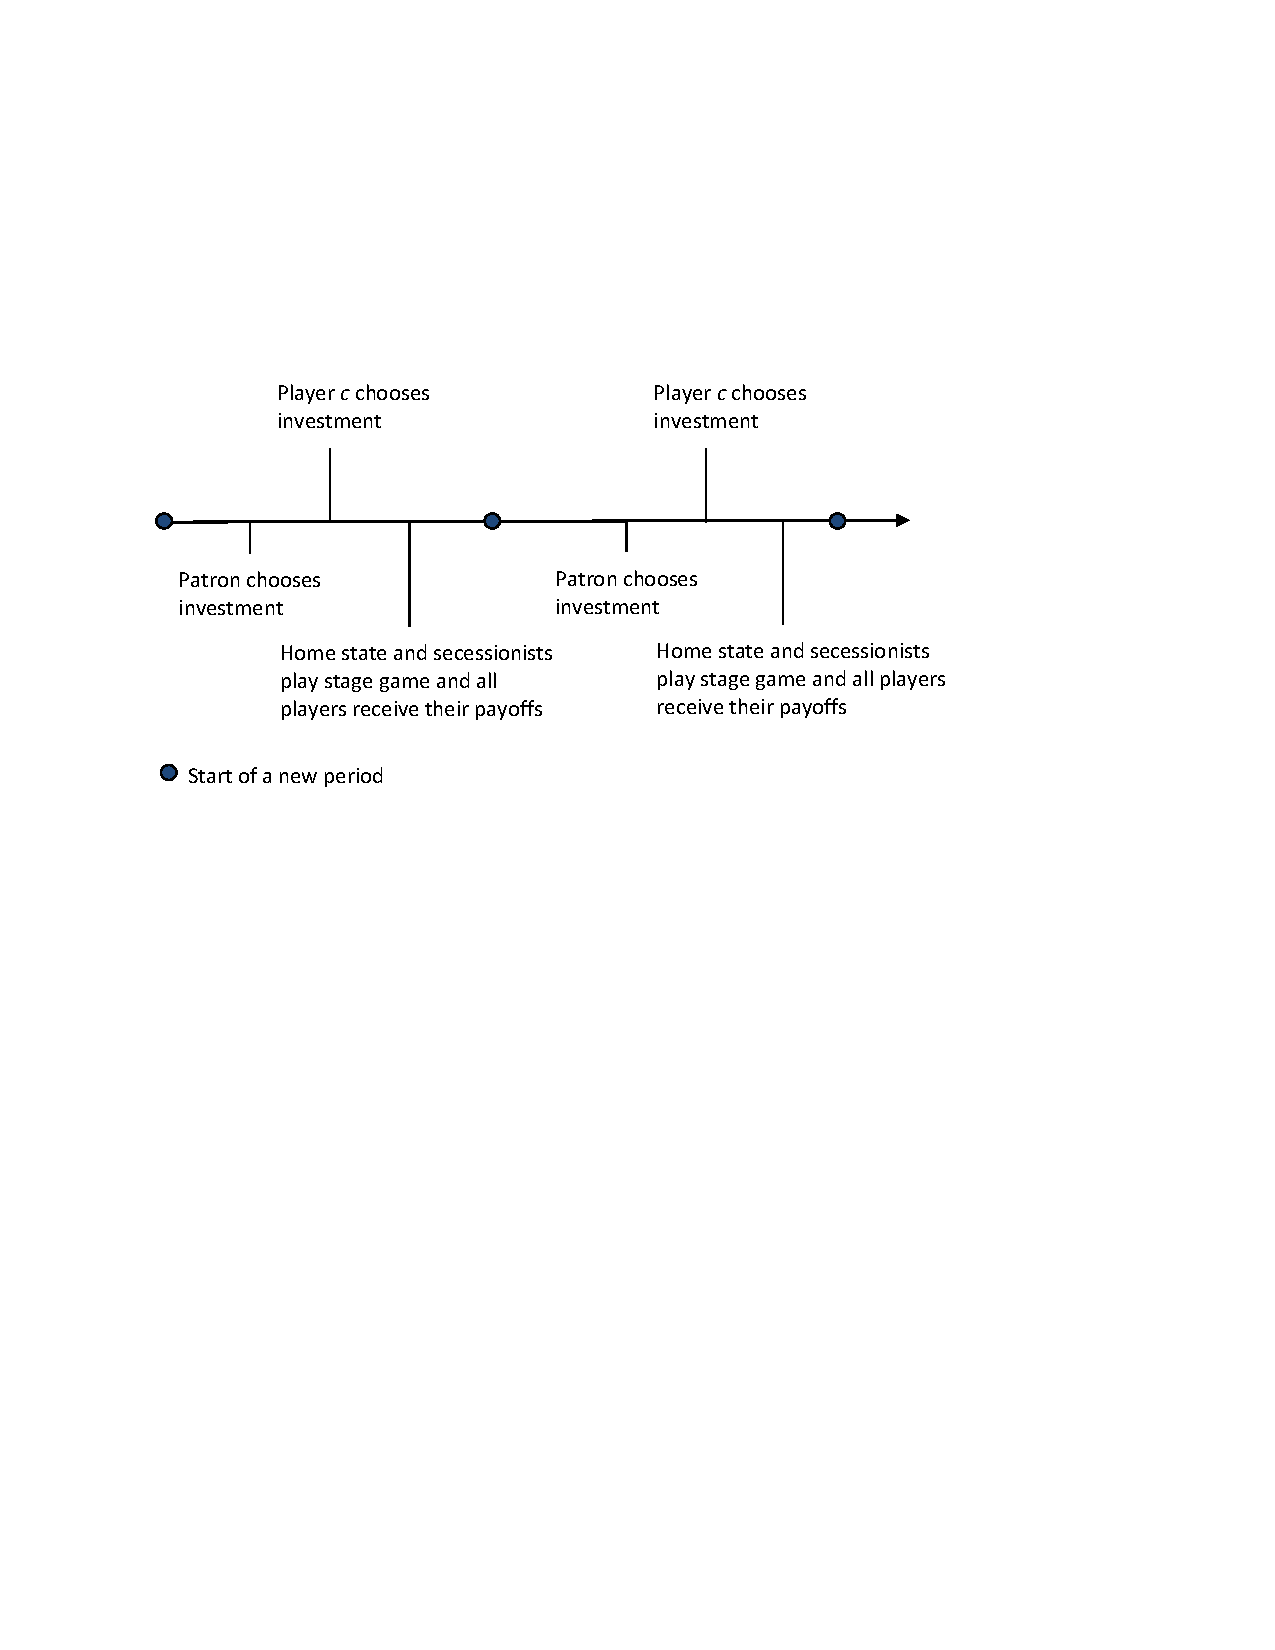
\includegraphics{Timeline2.pdf}
\caption{Timeline}
\end{figure}

\newpage

\begin{center}
\begin{tabular}{|  c| c | c | c |} 
\hline
  $g\downarrow$,     $ s\rightarrow$  & Fight & Status Quo &Cede \\ \hline
	Fight & $p_g W_g^t + p_s L_g^t - \zeta_g, p_s W_s^t + p_g L_s^t - \zeta_s$ &$p_g W_g^t + p_s L_g^t - \zeta_g, p_s W_s^t + p_g L_s^t - \zeta_s$&$W_g^t, L_s^t$ \\ \hline
	Status Quo& $p_g W_g^t + p_s L_g^t - \zeta_g, p_s W_s^t + p_g L_s^t - \zeta_s$& $\bm{Q_g^t, Q_s^t}$ &$W_g^t, L_s^t$ \\ \hline
	Cede&$L_g^t, W_s^t$& $L_g^t, W_s^t$ &$\bm{Q_g^t, Q_s^t}$ \\ \hline
 \multicolumn{4}{c} {Figure 2: Stage Game Payoffs}\\ 
\end{tabular}
\end{center}

\newpage
\begin{center}
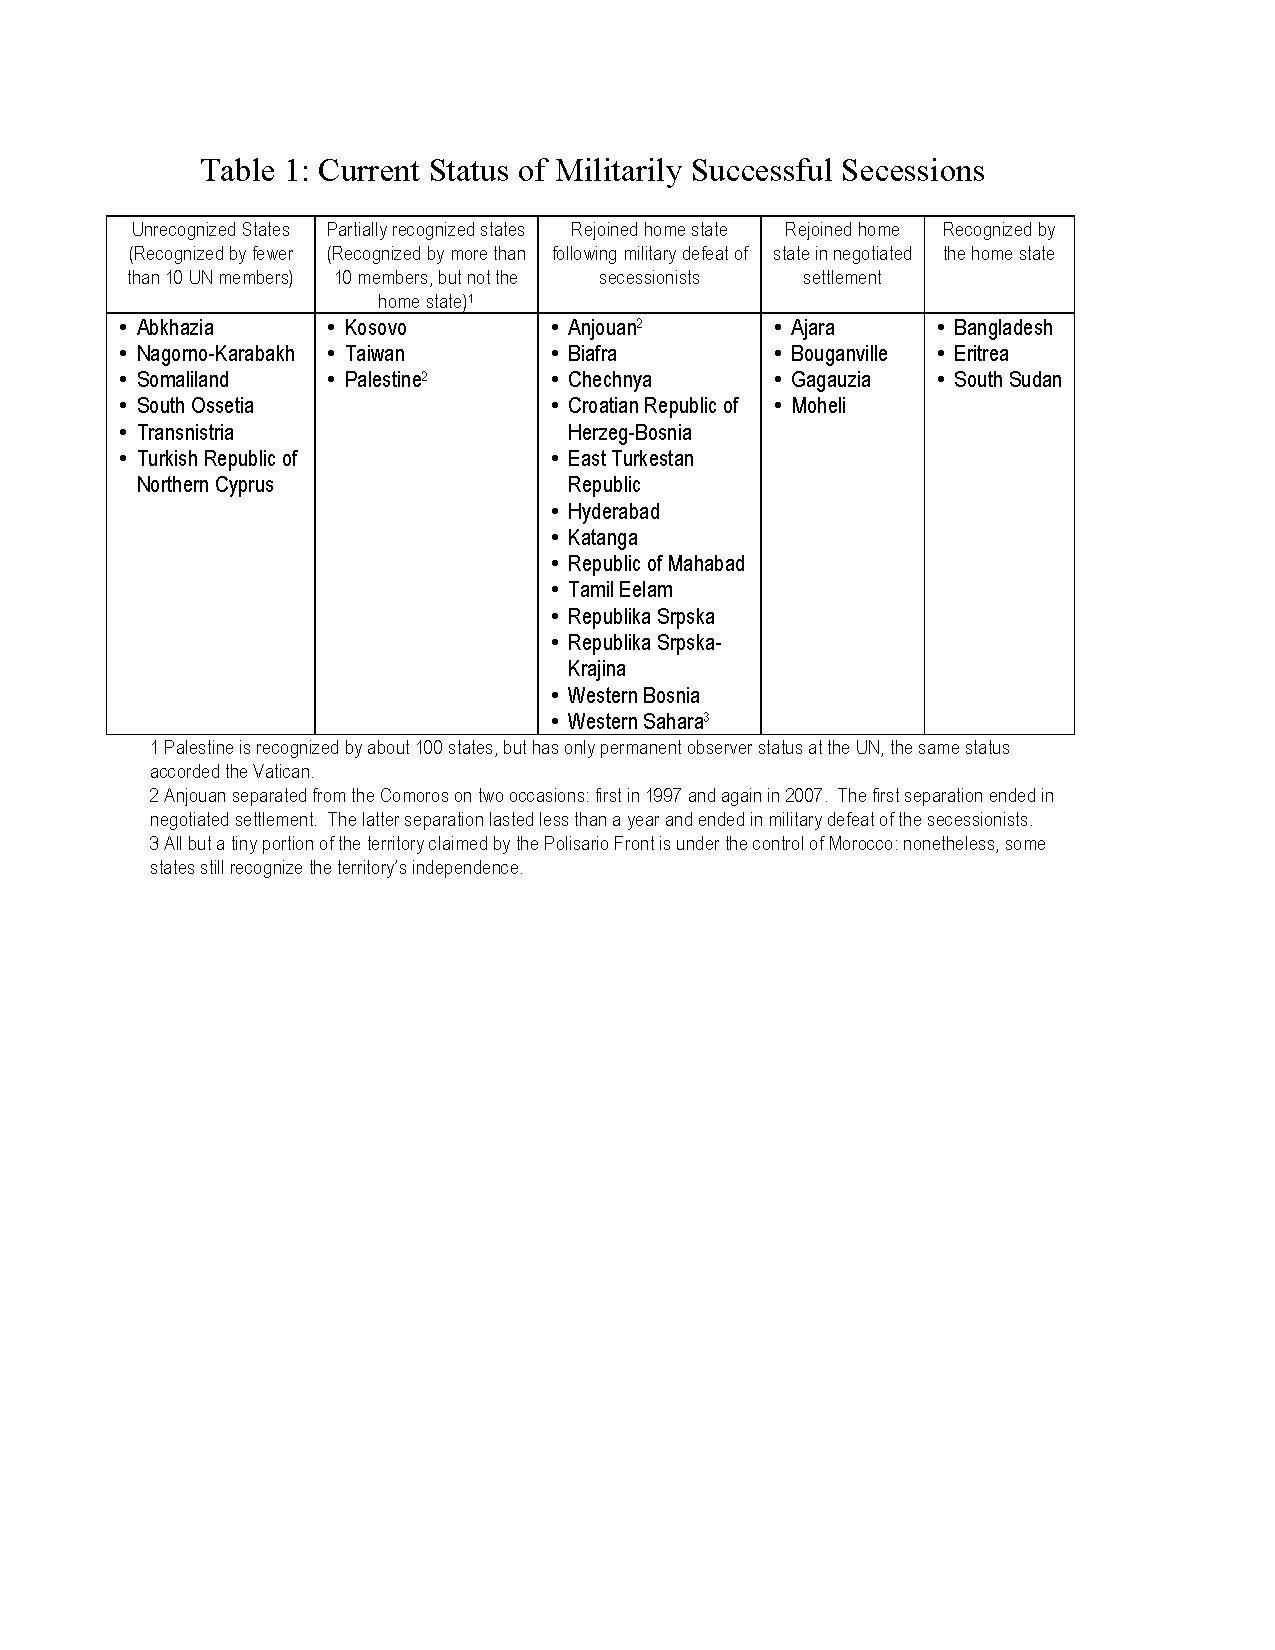
\includegraphics[width=6.25in]{Table_1_082214.pdf}
\end{center}


